\chapter{Literature Review}\label{sec:lit_review}

The aim of this section is to review the available literature in the areas of aerospace certification requirements, fatigue and damage tolerance analysis, linear-elastic fracture mechanics, and computational fracture mechanics. Aerospace certification requirements are first reviewed, in order to give context on the necessity of crack propagation calculations within the aerospace sector. An overview of fatigue and damage tolerance analysis is then provided, followed by a section on linear-elastic fracture mechanics, which introduces the theoretical basis for the software implementation. Finally, the section on computational fracture mechanics discusses the methods available for the implementation of the software.

\newpage
\section{Aerospace Certification Requirements}\label{sec:cert_req}

As discussed in \S\ref{sec:background}, fatigue and damage tolerance are critical factors influencing structural design in the civil aerospace sector. The fatigue and damage tolerance requirements that must be met in order for a large civil aircraft to be certified within Europe are defined in EASA Regulation CS \S25.571 -- 'Damage tolerance and fatigue evaluation of structure' \cite{noauthor_easy_2023}. These regulations have changed and developed over time, as new findings have been obtained from research, experience, and investigations of structural failures due to fatigue. There are four main approaches that have been used over the past century, all of which still applied today to various parts of a modern airframe.

\subsubsection*{Safe-Life (Safety by Retirement)}

This is the oldest and most conservative approach. Under this approach, a structure is designed such that the chance of crack initiation occurring within a specified service life is almost zero, using a combination of load spectra, physical testing, and factors of safety. The structure is retired once this service life has been reached, regardless of its actual condition. This approach has the highest margin of safety, but leads to higher costs and lower performance due to a combination of unnecessary weight, and potentially retiring components which still have a significant amount of life remaining. The safe-life approach has been superseded in most cases, but is still used for heavily-loaded components where the inspection of cracks before they become critical can be difficult \cite{lazzeri_comparison_2002}.

\subsubsection*{Fail-Safe (Safety by Design)}
    
The fail-safe approach was developed in order to remedy a key failing with the safe-life approach {-} namely that if a safe-life structure were to fail, the results can be catastrophic due to the fact that there is no redundancy considered within the approach. The key argument of the fail-safe approach is that a structural component should have a redundant load path -- a secondary component that can temporarily take the load of a failed component until the structure is inspected and the failed component either repaired or replaced \cite{schijve_load_2009}.
 
\newpage
\subsubsection*{Damage Tolerance (Safety by Inspection)}
    
This approach relies on the regular inspection of components in order to detect cracks and replace components before failure occurs. An initial crack is assumed to exist in a component at the beginning of its life, and fracture mechanics principles are used to calculate the rate of crack growth, and the point at which failure will occur. These values are then used to set an inspection threshold and repeat inspection intervals, to ensure that the component will be expected in the interval between the crack becoming detectable and the crack becoming critical, at which point the component will be repaired or replaced \cite{schijve_load_2009}.
    
\subsubsection*{Widespread Fatigue Damage (WFD)}

This is a relatively new requirement for aircraft, the introduction of which was necessary as the age of in-service aircraft grew over time. WFD refers to the possibility of multiple small cracks developing within different places within the structure. This can either be multi-side damage (MSD) for cracks present within different areas of the same structure, or multi-element damage (MED) for cracks present within similar adjacent structural elements. A limit of validity (LOV) must be defined for an aircraft, which is the limit at which available engineering data can demonstrate that WFD will not occur in the aircraft structure. The data may include test evidence, analysis, in-service data, and teardown inspection results of high-life aircraft \cite{anderson_fracture_2017}.
    
\newpage
\section{Fatigue \& Damage Tolerance Analysis}\label{sec:fdt_analysis}

The analysis approaches used within the civil aerospace sector to demonstrate compliance with the previously discussed certification requirements can be broadly split into fatigue analysis, and damage tolerance analysis. Pure fatigue analysis is used to demonstrate a structure's compliance with the safe-life or fail-safe requirements, while additional damage tolerance analysis is used to demonstrate a structure's compliance with the damage tolerance and widespread fatigue damage requirements. Most primary structures are required to be damage tolerant, and are therefore subjected to both fatigue and damage tolerance analysis.

\subsection{Fatigue Analysis}

Fatigue analysis is used to demonstrate compliance for structures that fall under the certification classification of safe-life or fail-safe. The key output of a fatigue analysis is a factored fatigue life for a structural component, given in flight cycles (FC). An unfactored fatigue life is the number of aircraft ground-air-ground (GAG) cycles that a component can be demonstrated to withstand before any crack initiation occurs -- assuming that the as-manufactured component was pristine and free of any cracks. This is multiplied by some factor of safety (usually either three or five) in order to produce the factored fatigue life. Fatigue analysis requires several key inputs, including data on the component's loading, geometry, and material, along with physical test data \cite{schijve_load_2009}.

\subsubsection{Load Spectra}\label{sec:load_spectra}

The load spectrum of an aircraft is a statistical representation of the series of cyclic loads that the average aircraft of that type will be subjected to during a typical flight cycle. Various load types are considered, including ground loads, cruise flight loads, manoeuvre loads, gust loads, and pressurisation loads. The load spectrum is created from a combination of computational methods, statistical analysis, and physical testing such as wind tunnel testing. It can further be tuned using flight test data, once it becomes available. The load spectrum is used along with a global finite element model (GFEM) in order to determine the individual loads on each component, which are then used to calculate individual stresses for each component. Finally, techniques such as the rainflow counting algorithm are used to sum up the effects of the individual loading cycles, and produce a single stress value that can be used to calculate the fatigue life for a component {-} this is known as the fatigue equivalent stress, or $S_{EQ_{FAT}}$ \cite{schijve_load_2009}.

\subsubsection{Geometry}

In order to convert the global aircraft loads into local component stresses, geometry is a key consideration. The most critical geometric influence on the fatigue life is the stress concentration factor (SCF). The stress concentration factor is a dimensionless measure, which is a ratio between the local stresses observed at a geometric feature {-} for example, a hole, fillet, or radii {-} and the remote stress observed in a plain area of the component. The stress concentration factor can be calculated using empirical data -- such as those available in\ \cite{pilkey_petersons_2008} -- or using linear-elastic finite element models. Stress concentrations are significant in fatigue analysis as they act as preferential sites for crack initiation, and can significantly reduce the fatigue life of a component.

\subsubsection{Material Properties}

Material properties are also a significant contributor to the fatigue life of a component, as materials differ significantly in their resistance to fatigue. Fatigue properties of a material are usually captured within a stress-life curve (S-N curve), which plots the applied fatigue stress versus the number of cycles to failure for a material. Values for this curve are generally obtained via coupon tests of the material in question, performed at various stress levels. The domain of most interest for aerospace structures is the high-cycle fatigue regime, which covers from around $10^3$ cycles up to around $10^6$ cycles. Factors such as the R-ratio, size effect, and surface finish of the coupons must be considered in order to be able to apply the results of the coupon testing accurately to the actual structure.

\subsubsection{Fatigue Life Calculation}

Using the available loading, geometry, and material data, an unfactored fatigue life can be calculated for the component. Safety factors are then applied to this to create a factored fatigue life. The magnitude of the safety factor used is dependent on the structure being analysed and the available test evidence. Finally, the factored fatigue life can be compared to the design service goal (DSG) of the aircraft -- which is the number of flight cycles that the aircraft is being certified for. If the factored fatigue life is greater than the design service goal, then the analysed component has an extremely low risk of crack initiation during the lifetime of the aircraft, and can therefore be safely used. If the factored fatigue life is less than the design service goal, then it may be necessary to introduce inspections for the component into the maintenance plan, or replace the component midway through the aircraft's service life

\newpage
\subsection{Damage Tolerance Analysis}

Damage tolerance analysis is used to demonstrate the compliance of a structure with the damage tolerance and widespread fatigue damage certification requirements. In contrast to fatigue analysis, damage tolerance analysis is mainly concerned with the growth rate of pre-existing cracks in a structure, and the determination of inspection intervals which enable these cracks to be detected and mitigated before reaching the critical length that will lead to structural failure. Linear-elastic fracture mechanics (LEFM) is the key theoretical basis for damage tolerance analysis, which is discussed in more detail in \S\ref{sec:lefm}. Damage tolerance analysis involves determining the likely sizes and locations of any flaws, calculating the rate at which that they will grow, and determining the necessary inspection interval to ensure they are detected in a timely manner.

\subsubsection*{Initial Flaws}

Damage tolerance analysis presumes that small flaws (i.e. cracks) exist within any structure, which are present from the beginning of the service life of the aircraft. The sizes and prevalences of these flaws are estimated based on the statistical analysis of quality inspection data obtained during manufacture and in service, while knowledge of non-destructive testing (NDT) techniques is used to determine the likelihood of detecting cracks at a given size. The aim of this process is to conservatively estimate the maximum size of flaw which is realistically able to escape the manufacturing environment, without being discovered during a quality inspection. This is known as a rogue flaw, and a value of 0.05" or 1.27 mm is commonly used \cite{davidson_405_2003}. A stress survey is then performed using a GFEM in order to select a primary crack location for a structure based on its criticality. This process takes into account factors such as loading and geometry in order to determine the location at which the presence of a crack would lead to the failure of the structure within the lowest number of loading cycles. A secondary location is also selected, which is generally the redundant structure which would be subjected to the redistributed load upon failure of the primary structure. At the secondary location, a smaller crack is assumed to be present -- this is known as a quality flaw, and a value of 0.005" or 0.127 mm is used -- one order of magnitude less than the rogue flaw. These assumptions represent a conservative "worst-case" scenario for crack propagation, where cracks are present at both the most highly stressed location, along with its redundant structure. An example of this for a skin-stringer panel section is presented in Figure \ref{fig:primary_secondary}.

\begin{figure}[H]
	\centering
	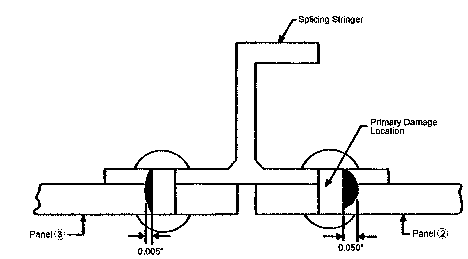
\includegraphics[width=10cm]{primary_secondary.png}
	\caption{Primary and secondary damage locations within a skin-stringer section. The primary location has a 0.05" rogue flaw and the secondary location has a 0.005" quality flaw. The flaws impact both the skin panel and the stringer, as both are drilled during the same operation \cite{afgrow_dtdhandbook_nodate}.}
	\label{fig:primary_secondary}
\end{figure}

\subsubsection*{Crack Growth and Failure}

Once the primary and secondary damage locations have been selected, the crack propagation life of the structure is then calculated -- this is the number of flight cycles that causes the crack to grow to the length necessary to cause failure of the structure. Most aircraft structures are thin-walled, and therefore can be idealised as two-dimensional. Well-established analytical methods are then available to calculate the stress intensity factor (SIF) for these idealised structures -- this is discussed in further detail in \S\ref{sec:sif}. These analytical methods are not usually applicable to thicker three-dimensional structures, and therefore numerical approaches must be used (discussed in further detail in \S\ref{sec:comp_fracture}). The loading of the structure is determined using the approach described in \S\ref{sec:load_spectra}, which is then used to calculate the crack propagation equivalent stress -- $S_{EQ_{CP}}$. This parameter is similar to $S_{EQ_{FAT}}$, but additionally considers the angle of crack growth relative to the direction of applied loading. Once an accurate stress intensity factor has been obtained, the rate of crack growth can then be determined using the Paris-Erdogan equation (Equation \ref{eq:paris_law}). This process is repeated by extending the crack, and recalculating the stress intensity factor for this slightly longer crack. At each step, the limit stress ($\sigma_{limit}$) -- which is the maximum stress that the structure is likely to be subjected to during its entire service life -- is compared to the residual strength of the component. A visualisation of the crack growth curve vs the residual strength of the structure is presented in Figure \ref{fig:residual_strength}. When the stress intensity factor of the crack under an applied stress of $\sigma_{limit}$ reaches the critical stress intensity factor of the material ($K_{IC}$), the structure fails. The length of the crack at this point is known as the critical crack length ($a_{crit}$) \cite{afgrow_dtdhandbook_nodate-1}.

\begin{figure}[H]
	\centering
	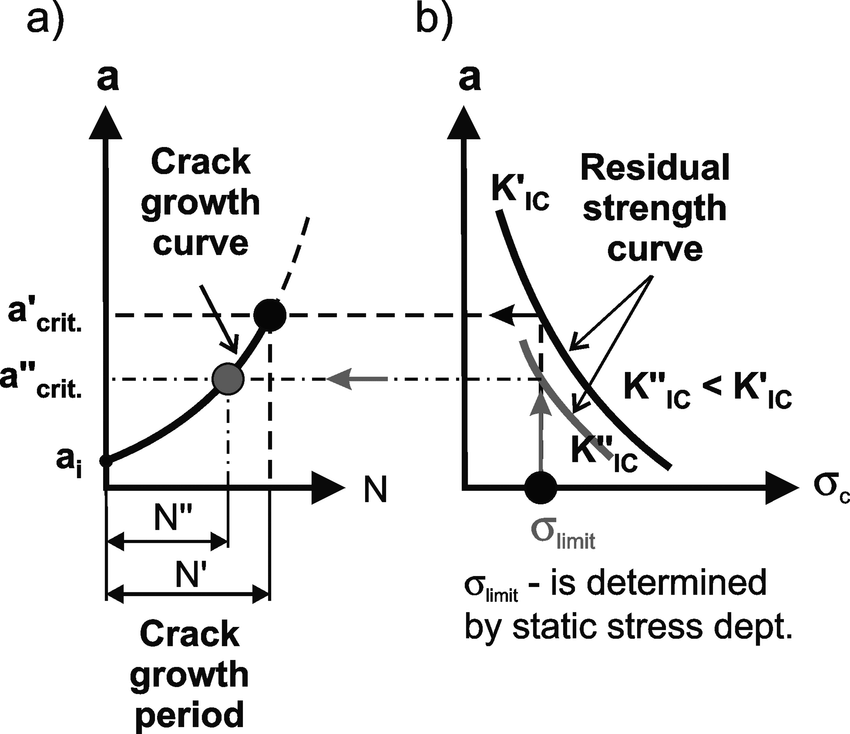
\includegraphics[width=10cm]{residual_strength.png}
	\caption{Diagram showing the crack growth curve (a) along with the residual strength curve (b). When the stress intensity factor of the crack under an applied stress of $\sigma_{limit}$ reaches the critical stress intensity factor of the material, the structure fails \cite{dzidowski_effect_2013}.}
	\label{fig:residual_strength}
\end{figure}

\subsubsection*{Threshold and Inspection Intervals}

The previously calculated crack propagation lives can then be used to determine the inspection threshold and inspection intervals for the analysed structure. The inspection threshold is the point at which the first inspection of the structure is required, while the inspection intervals are the points at which repeat inspections are required. For example, a structure with an inspection threshold of 24,000 FC and an inspection interval of 6,000 FC would require an initial inspection once the aircraft has completed its first 24,000 flight cycles, and additional inspections after every subsequent 6,000 flight cycles. The inspection threshold is generally half of the structure's factored fatigue life, while the inspection intervals are determined based on the crack propagation lives determined via damage tolerance analysis \cite{gallagher_damage_2005}.

The parameters of interest when determining the inspection intervals are $a_{crit}$, $a_{det}$ $N_{primary}$ and $N_{secondary}$. The critical crack length ($a_{crit}$), is the crack length at which the secondary damage location fails, while ($N_{primary}$) and ($N_{secondary}$) are the number of crack growth cycles to failure for the primary and secondary damage locations respectively. The final parameter ($a_{det}$) is the detectable crack length, which is the length at which the crack in the primary damage location becomes detectable via the inspection method specified for the structure. The selected method differs depending on the accessibility and visibility of the structure in question.

The inspection intervals are determined based on the number of cycles that occur between the crack at the primary location becoming detectable (when the crack length at the primary location reaches $a_{det}$), and the crack in the secondary location causes failure of the component (when the crack length at the secondary location reaches $a_{crit}$). The interval between these two parameters provides a window of opportunity, where a crack can be reliably detected, but before structural failure has occurred. The inspection interval is then divided by a safety factor of two. This provides two opportunities to detect the crack, to account for a the possibility of an inspection failing to detect a crack that should have been detected. Figure \ref{fig:damage_tolerance_chart} demonstrates the period of safe crack growth that is used to determine the damage tolerance inspection intervals for an aircraft structure. Note that the rate of crack growth at the secondary location increases once the primary member has failed, due to load being distributed from the primary to the secondary location \cite{tomblin_review_1999}.

\begin{figure}[H]
    \centering
    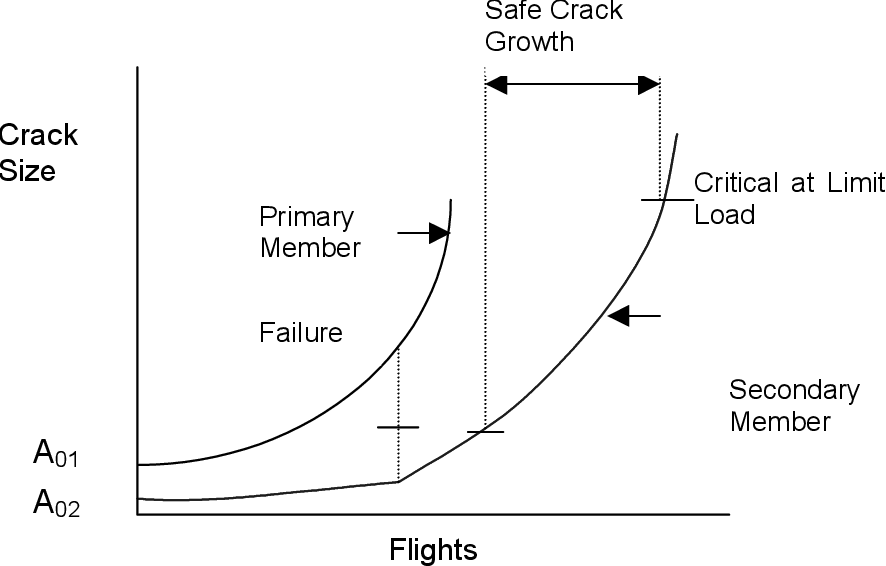
\includegraphics[width=14cm]{damage_tolerance_chart.png}
    \caption{Crack propagation chart showing the growth of a crack at a primary and secondary location as the number of flight cycles increase. Once the primary location has failed, redistributed load accelerates the growth of the crack at the secondary location. \cite{tomblin_review_1999}.}
    \label{fig:damage_tolerance_chart}
\end{figure}

\newpage
\section{Linear Elastic Fracture Mechanics}\label{sec:lefm}

Linear Elastic Fracture Mechanics (LEFM) is a fundamental framework within the field of fracture mechanics. The key underlying assumption of LEFM is that the overall deformation of a cracked body is linear-elastic. This means that the plastic zone at the crack tip is small relative to the length of the crack, and that the stress state at the crack tip can be accurately described using only the elastic stresses in the material. LEFM was first developed by Griffith in 1920, via the application of the first law of thermodynamics to the problem of crack formation and propagation \cite{griffith_vi_1921}.

The first law of thermodynamics states that energy must always be conserved -- this implies that when a system moves from a non-equilibrium state to an equilibrium state, there must be no net increase in energy. Griffith applied this principal to fracture mechanics in the form of a global energy balance -- where the elastic energy stored in a stressed body was balanced against the increase in surface energy necessary to create new crack surfaces in that body.

The growth of a crack within a body results in an increase in the surface energy of that body -- this is because the creation of new crack surfaces requires work to be done in order to break atomic bonds at those surfaces. The creation of new surfaces relaxes the stresses within the body, and therefore reduces the elastic potential energy at the crack faces. Griffith's model stated that crack extension would occur when the elastic potential energy stored in a cracked body was equal to the increase in the surface energy of the body due the extension of the crack. Restated, crack extension would occur at the point where there was no net change in the total energy of the body due to the extension of the crack.

Equation \ref{eq:griffith} presents Griffith's equation for a through-thickness crack in an infinitely wide plate subjected to a remote tensile stress. Griffith's model provided good agreement with experimental data for brittle materials. However, the surface energy predicted by the model was unrealistically high for ductile materials.

\begin{equation}
	\sigma_f = \sqrt{\frac{2 E \gamma_s}{\pi a}}\label{eq:griffith}
\end{equation}

\begin{itemize}
	\item $\sigma_f$ is the tensile stress necessary to cause fracture of the material.
	\item $a$ is the crack length.
	\item $E$ is the elastic modulus.
	\item $\gamma_s$ is the surface energy per unit area.
\end{itemize}

\newpage
Irwin later modified Griffith's model to account for the effects of localized plastic deformation within ductile materials, and therefore increase the predictive accuracy of the model for these materials. Irwin found that in ductile materials, a plastic zone develops at the tip of the crack, resulting in additional work being done and heat being dissipated during the process of crack extension. Irwin added an additional term ($\gamma_p$) to Griffith's equation, which is the plastic work done per unit area of surface created. Equation \ref{eq:irwin} presents Irwin's corrected equation for fracture stress.

\begin{equation}
	\sigma_f = \sqrt{\frac{2 E (\gamma_s + \gamma_p)}{\pi a}}\label{eq:irwin}
\end{equation}
 
Irwin later proposed an energy approach for fracture, known as the strain energy release rate \cite{irwin_onset_1956}.  This was essentially equivalent to Griffith's model, but was revised into a more convenient form. Irwin defined the strain energy release rate ($G$), which is a measure of the decrease in total potential energy per increase in fracture surface area. Equation \ref{eq:strain_energy} gives the formula for the strain energy release rate $G$, for a wide plate under plane stress conditions with a centre crack of length $2a$ and an applied tensile stress of $\sigma$. Crack extension occurs when $G$ reaches the critical value of $G_c$, where $G_c$ is a measure of the fracture toughness of the material.

\begin{equation}
	G = \frac{\pi \sigma^2 a}{E}\label{eq:strain_energy}
\end{equation}

\newpage
\subsection{Stress Intensity Factor}\label{sec:sif}

The stress concentration factor ($K_t$) is used to characterise stress distributions around features such as notches and holes, and is defined as the ratio between the stress in the immediate vicinity of the feature, and the stress at some point in the bulk material, remote from any features. However, $K_t$ ceases to become a meaningful concept near the tip of a sharp crack -- as the radius of the crack tip approaches zero, the stress approaches a value of infinity. The definition of the stress intensity factor (SIF) by Irwin was therefore a key development in the field of linear-elastic fracture mechanics, as it enabled the stress state at the tip of a sharp crack to be characterised using a single parameter \cite{irwin_analysis_1957}. For a polar coordinate system defined with the origin at the crack tip, it can be shown that the stress field in any linear elastic cracked body can be represented by Equation \ref{eq:sigma_ij} \cite{anderson_fracture_2017}.

\begin{equation}
	\sigma_{ij} = \left(\frac{k}{\sqrt{r}}\right) f_{ij}(\theta) + \sum_{m=0}^{\infty} A_m r^{\frac{m}{2}} g_{ij}^{(m)}(\theta)\label{eq:sigma_ij}
\end{equation}

\begin{itemize}
	\item $\sigma_{ij}$ is the stress tensor.
	\item $r$ and $\theta$ are parameters defining the polar coordinate system presented in Figure \ref{fig:2d_3d_cracks_hellen}.
	\item $k$ is a constant.
	\item $f_{ij}$ is a dimensionless function of $\theta$.
	\item $A_m$ is the amplitude.
	\item $g_{ij}^{(m)}$ is a dimensionless function of $\theta$ for the $m$th term.
\end{itemize}

The parameters in the second part of the expression are dependent on the specific configuration of the problem being analysed. However, the first part of the expression is proportional to $\frac{1}{\sqrt{r}}$ for any possible geometry. As $r$ approaches zero, the first part of the expression approaches infinity, while the second part approaches zero. Therefore, Equation \ref{eq:sigma_ij} demonstrates that the stress near the crack tip is proportional to the $\frac{1}{\sqrt{r}}$ term, regardless of the configuration of the cracked body.

\begin{figure}[H]
	\centering
	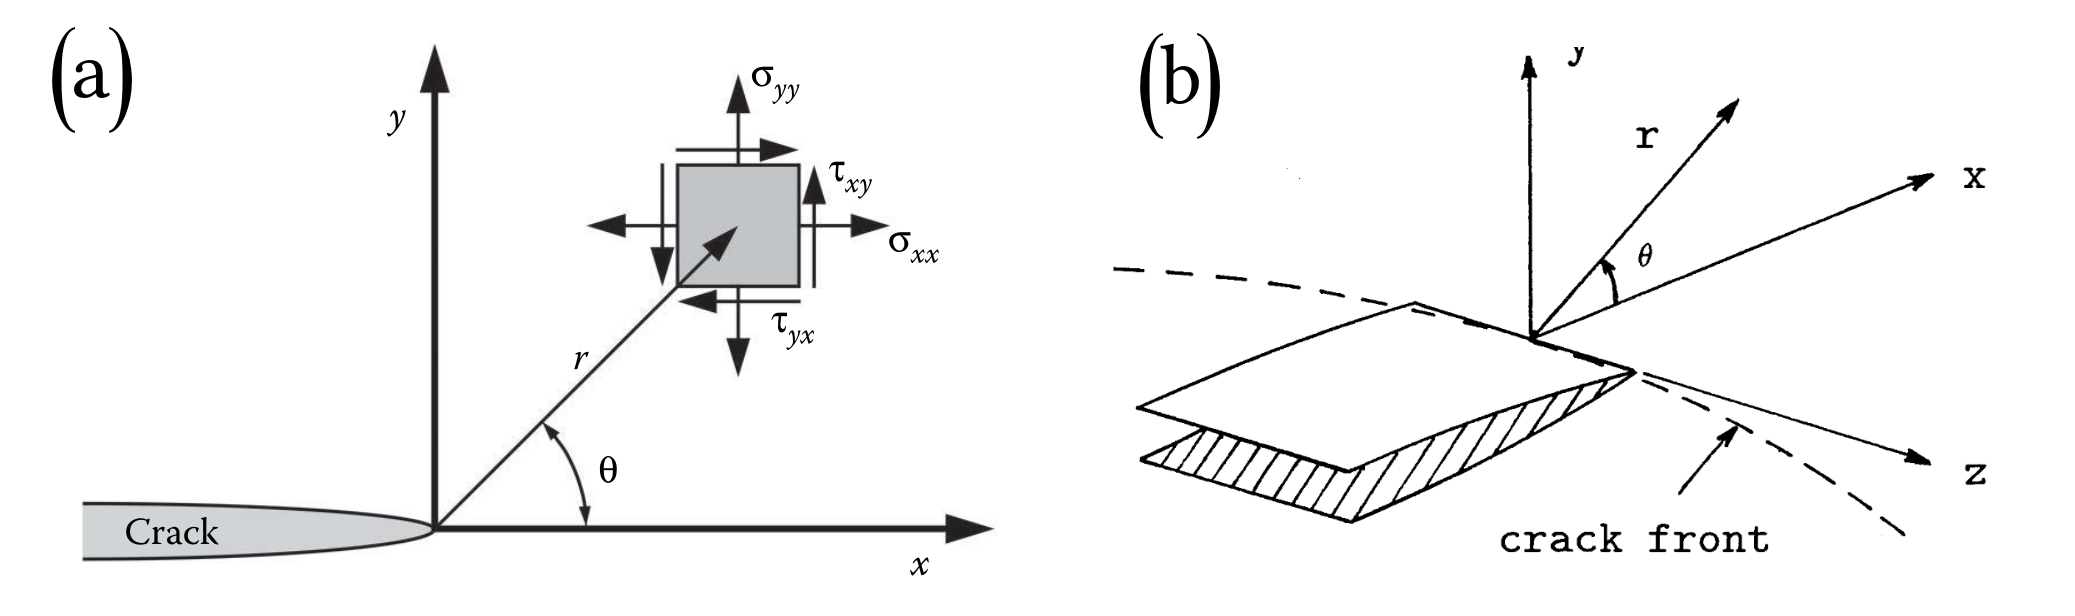
\includegraphics[width=15cm]{2d_3d_cracks_hellen.png}
	\caption{A diagram showing crack tip geometry in two dimensions (a) and three dimensions (b), showing the polar coordinate system constructed using $r$ and $\theta$.\ \cite{hellen_how_2001}.}
	\label{fig:2d_3d_cracks_hellen}
\end{figure}

\newpage
Equation \ref{eq:sigma_ij} may then be used to define the stress intensity factor ($K$) by introducing a $\pi$ term for the sake of convenience, as given by Equation \ref{eq:k_to_K}. The proportionality constants $k$ and $f_{ij}$ are dependent on the configuration of the problem, such as the geometry, loading, and boundary conditions. This therefore implies that $K$ is also dependent on these factors.

\begin{equation}
	K = k \sqrt{2 \pi}\label{eq:k_to_K}
\end{equation}

The stress intensity factor can then be obtained in terms of the applied stress and the crack length -- this is presented in Equation \ref{eq:sif}. The parameter $\beta_{i}$ is a shape factor that accounts for the configuration of the specific problem, for the specific loading mode in question. For a straight crack of length $2a$ which  is embedded in an infinite plate and subjected to a uniform stress of $\sigma$ acting perpendicular to the crack, $\beta$ is equal to one. For other configurations, $\beta$ must be determined via analytical equations, numerical methods, or physical testing.

\begin{equation}
	K_{i} = \beta_{i}\sigma \sqrt{\pi a}\label{eq:sif}
\end{equation}

\begin{itemize}
	\item $K_i$ is the stress intensity factor for the crack loading mode $i$.
	\item $\beta_{i} $ is a dimensionless shape factor relating to the specific configuration of the problem, for the crack loading mode $i$.
	\item $\sigma$ is the applied stress.
	\item $a$ is the crack length. 
\end{itemize}

Stress intensity factor solutions for many two-dimensional plane-stress configurations are readily available both within reference handbooks Sih \cite{sih_handbook_1973} and commercial software such as NASGRO and AFGROW. An example is presented in Figure \ref{fig:sif_solution}, which shows a SIF solution within NASGRO -- along with its limits of validity -- applicable to an edge crack in a finite plate. These solutions provide a method of quickly determining the stress intensity factor, without necessitating the comprehensive validation required when using a DFEM. However, most SIF solutions are only applicable to simplified and idealised geometry, and therefore they are not suitable for every problem. For example, the TC14 solution presented in Figure \ref{fig:sif_solution} is only valid for length-to-width ratios between 0.2 and 10. Obtaining the stress intensity factor for configurations which do not have solutions already available is more complex, and usually requires the use of finite element analysis. This is discussed further in \S\ref{sec:comp_fracture}.

\begin{figure}[H]
	\centering
	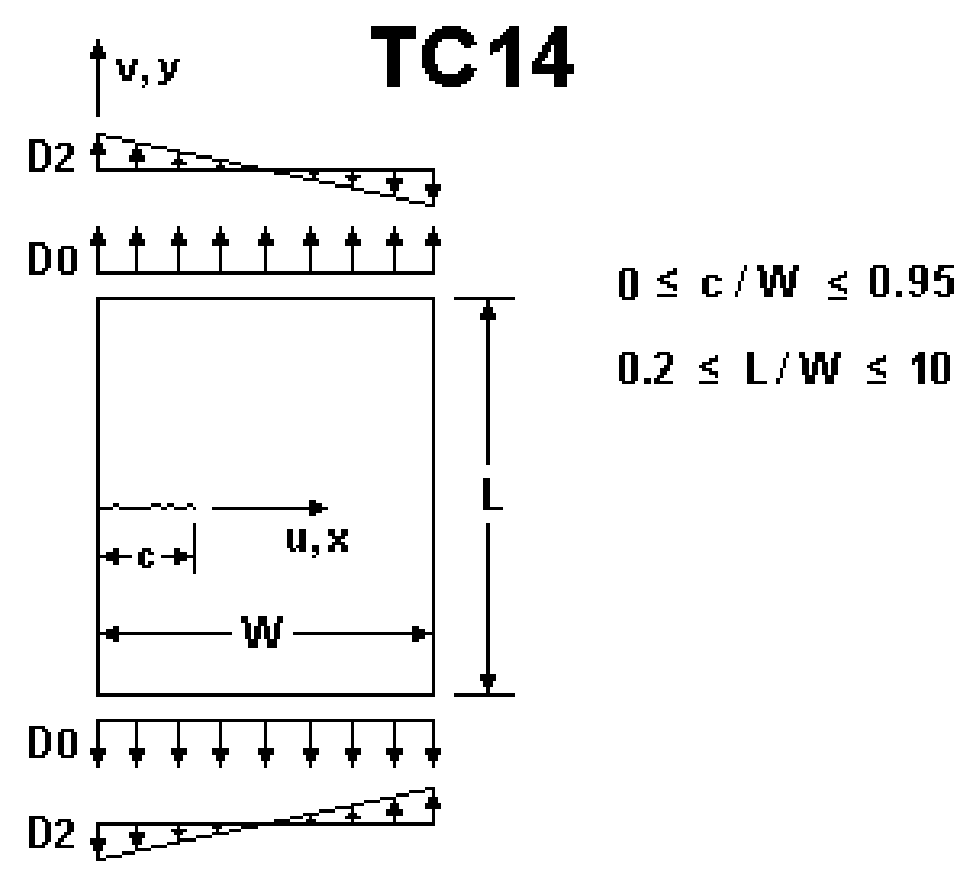
\includegraphics[width=9cm]{tc14_sif_solution.png}
	\caption{Diagram showing SIF solution TC14 from the NASGRO manual, which can be used to analyse through-thickness edge cracks within a finite plate \cite{nasgro_fatigue_2022}.}
	\label{fig:sif_solution}
\end{figure}

The rate of crack growth has been experimentally shown to be a function of the range of the stress intensity factor exhibited within a loading cycle. This is a critical relationship within aerospace damage tolerance analysis, as it allows the crack propagation life of a structure to be calculated using the stress intensity factor. This relationship is described by the Paris-Erdogan equation, presented as Equation \ref{eq:paris_law} \cite{anderson_fracture_2017}.

\begin{equation}
	\frac{da}{dN} = C(\Delta K)^m\label{eq:paris_law}
\end{equation}

\begin{itemize}
	\item ${da}/{dN}$ is the change in crack length per loading cycle.
	\item $\Delta K$ is the change in the stress intensity factor within the loading cycle, equal to ($K_{max} - K_{min}$).
	\item  $C$ and $m$ are material-specific properties which are obtained experimentally.
\end{itemize}

\newpage
\subsection{Crack Loading Modes}

Cracks may be subjected to three different types of loading, which are demonstrated in Figure \ref{fig:fracture_loading_modes_anderson}. Mode I loading occurs when the principal load is applied in the $y$ direction in order to open the crack - this is known as the opening mode. Mode II loading occurs when when an in-plane shear load is applied in the $x$ direction - this is known as the sliding mode. Finally, Mode III loading occurs when an out-of-plane shear load is applied in the $z$ direction - this is known as the tearing mode.

\begin{figure}[H]
	\centering
	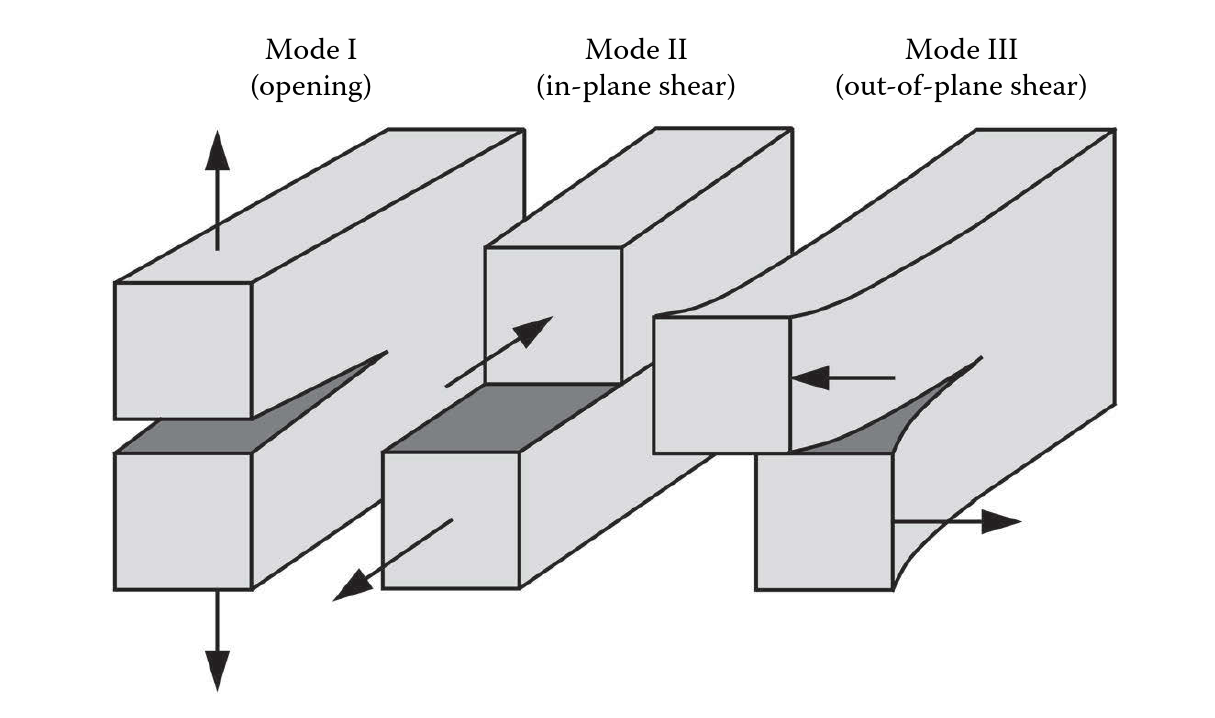
\includegraphics[width=11cm]{fracture_loading_modes_anderson}
	\caption{Diagram showing Mode I, Mode II, and Mode III crack loading\ \cite{anderson_fracture_2017}.}
	\label{fig:fracture_loading_modes_anderson}
\end{figure}

Separate expressions for the stress intensity factor can be defined for each mode of loading. These are given in Equations \ref{eq:k_i}, \ref{eq:k_ii}, and \ref{eq:k_iii} \cite{anderson_fracture_2017}.

\begin{equation}
	\lim_{r \rightarrow 0} \sigma_{ij}^{(I)} = \frac{K_{I}}{\sqrt{2 \pi r}} f_{ij}^{(I)} (\theta)
	\label{eq:k_i}
\end{equation}

\begin{equation}
	\lim_{r \rightarrow 0} \sigma_{ij}^{(II)} = \frac{K_{II}}{\sqrt{2 \pi r}} f_{ij}^{(II)} (\theta)
	\label{eq:k_ii}
\end{equation}

\begin{equation}
	\lim_{r \rightarrow 0} \sigma_{ij}^{(III)} = \frac{K_{III}}{\sqrt{2 \pi r}} f_{ij}^{(III)} (\theta)
	\label{eq:k_iii}
\end{equation}

Generally the mode of most concern when analysing crack propagation problems is Mode I, as this is the mode that occurs most frequently and produces the most damage. It has therefore received the most attention with regards to the research and development of damage tolerance methods. However, consideration of the other modes is still a significant factor, particularly when considering three-dimensional components which are made up of ductile materials and are subjected to multi-axial stresses. In these scenarios, a crack experiences a combination of different loading modes simultaneously -- this is known as mixed-mode fracture mechanics.

The principal of linear superposition can be used to calculate the sum the contributions of each loading mode to the overall stress tensor using Equation \ref{eq:stress_sum} \cite{anderson_fracture_2017}.

\begin{equation}
	 \sigma_{ij}^{(total)} = \sigma_{ij}^{(I)} + \sigma_{ij}^{(II)} + \sigma_{ij}^{(III)}\label{eq:stress_sum}
\end{equation}

The stress intensity factor is also specific to loading mode, and can also be superimposed via linear superposition. This is demonstrated by Equation \ref{eq:sif_superposition} \cite{anderson_fracture_2017}. This equation can be used to calculate the total stress intensity factor of a crack that is subjected to mixed-mode loading -- by calculating the stress intensity factor for each mode, and then summing the results. The process may also be performed in reverse, by calculating the total stress intensity factor for a crack, and then decomposing it into the separate stress intensity factors for each mode of loading. However, this is out of scope for this thesis, which focuses on a case study relating solely to Mode I loading.

\begin{equation}
	K_{total} = K_{I} + K_{II} + K_{III}\label{eq:sif_superposition}
\end{equation}

\newpage
\subsection{J-Integral}\label{sec:j-integral}

As discussed previously, the stress intensity factor is an extremely useful parameter which can be used to accurately calculate the crack propagation lives of structures. However, the available stress intensity factor solutions are mostly limited to two-dimensional idealisations, meaning that calculating the stress intensity factor for cracks in three-dimensional requires individual analysis using the finite element method. Therefore, a method of obtaining the stress intensity factor from the results of a finite element analysis is necessary. This is often accomplished via the use of the J-integral.

The J-integral was first described by Rice in 1968, and is an energy-based parameter which is closely related to the strain energy release rate ($G$) discussed briefly in \S\ref{sec:lefm}. The J-integral is a path-independent contour integral around the tip of a crack, and is defined in Equation \ref{eq:j-integral} \cite{rice_path_1968}.

\begin{equation}
	J = \int_{\Gamma} \left( W \, dy - T_i \frac{\partial u_i}{\partial x} \, ds \right)\label{eq:j-integral}
\end{equation}

\begin{itemize}
	\item $W$ is the strain energy density.
	\item $dy$ is an infinitesimal section taken perpendicular to the direction of crack growth.
	\item $T_i$ is the traction vector.
	\item $\frac{\partial{u_i}}{\partial{x}}$ is the rate of change of the displacement vector in the direction of crack growth.
	\item $ds$ is an infinitesimal section of a line integral around the crack tip.
\end{itemize}

The first term of the equation essentially captures the state of elastic deformation around the crack tip, and represents the energy stored in the stretching of the atomic bonds of the material. The second term captures the effects of the work done by external forces to create new free surfaces as the crack grows. Both terms together therefore quantify the total energy release rate, which encompasses the contributions from both elastic and plastic deformation of the material. As J-integral is able to capture the effects of plastic deformations, it can also be used to perform elastic-plastic fracture mechanics (EPFM) analysis -- where the plastic deformation around the crack tip is large relative to the crack length.

\begin{figure}[H]
	\centering
	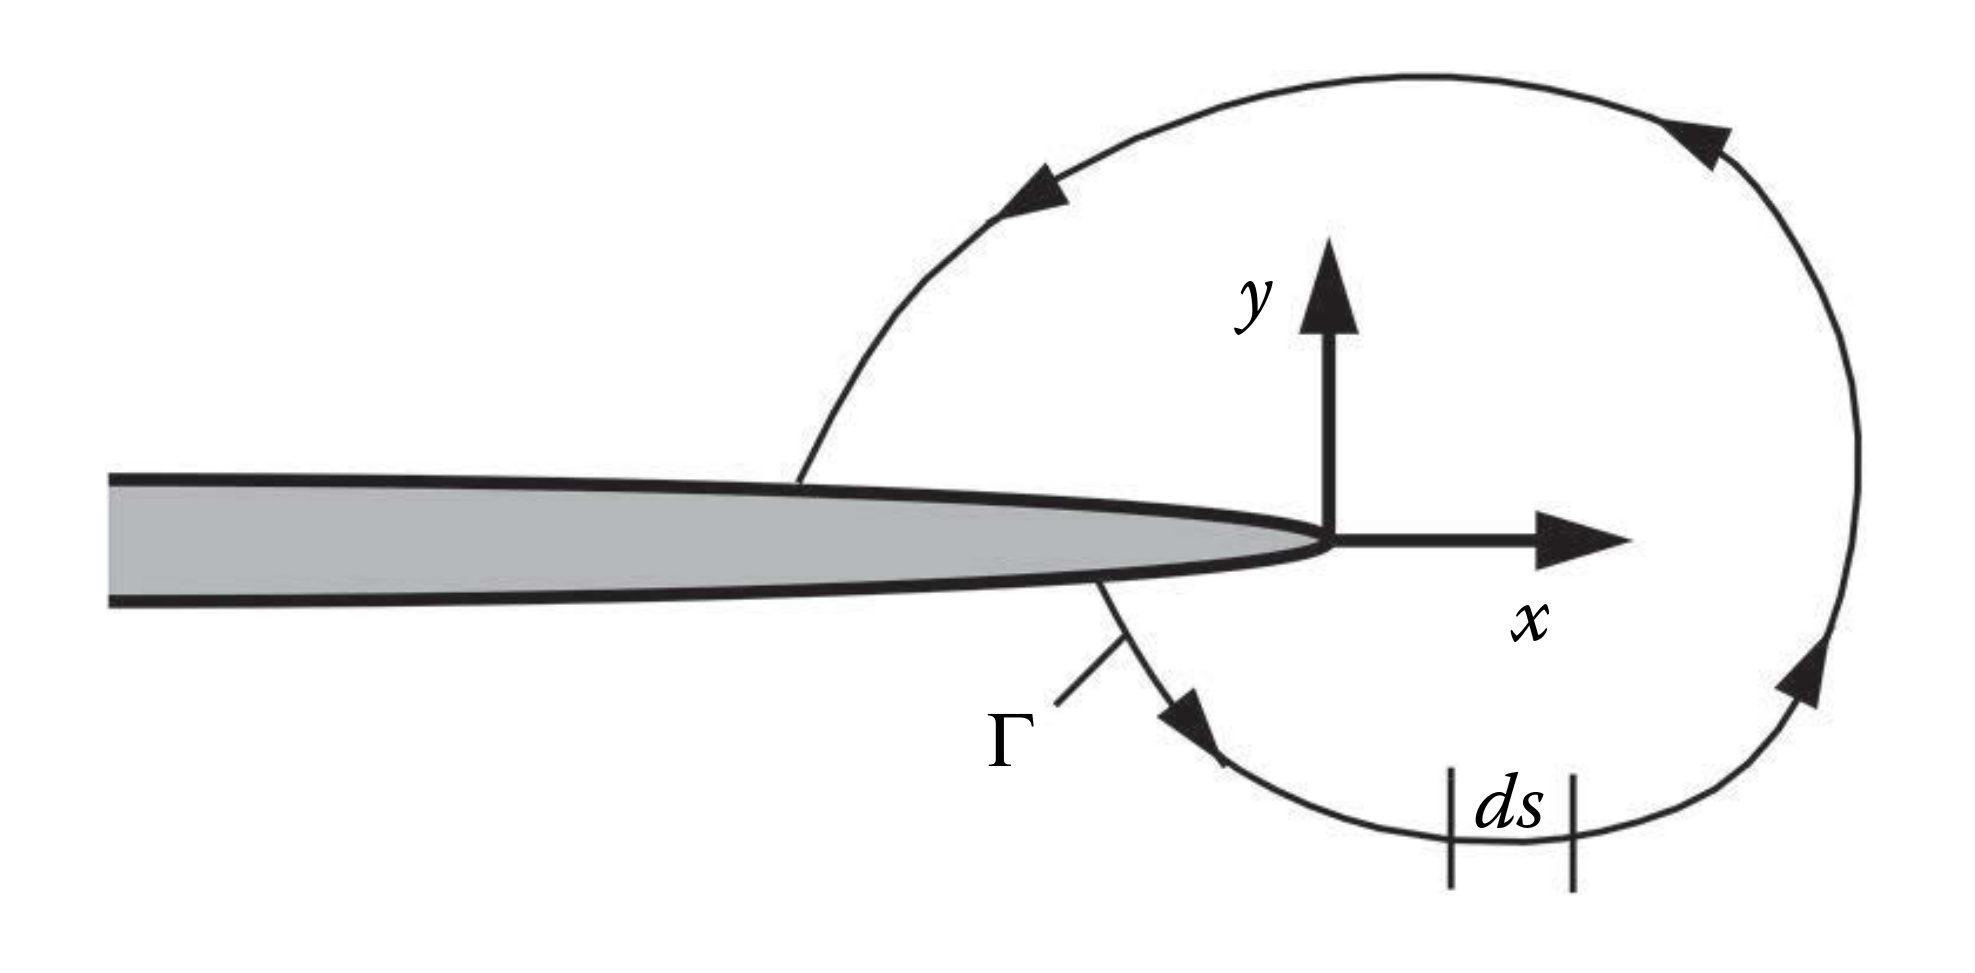
\includegraphics[width=10cm]{j-integral_diagram_anderson.png}
	\caption{Diagram of a crack, showing the closed contour $\Gamma$ that may be used to calculate J-integral\ \cite{anderson_fracture_2017}.}\label{fig:j-integral_diagram_anderson}
\end{figure}

For linear elastic materials, J-integral has been shown to be equal to the strain energy release rate ($G$) discussed in \S\ref{sec:lefm}. This means that the J-integral can be directly related to the stress intensity factor, which is the key piece of theory underpinning this thesis. This relationship is given in Equation \ref{eq:j-integral_sif}.

\begin{equation}
	J = G = \frac{K_I^2 + K_{II}^2}{E'} + \frac{K_{III}^2}{2 \mu}
	\label{eq:j-integral_sif}
\end{equation}

\begin{itemize}
	\item $E'$ is the effective elastic modulus of the material, which is equal to $E$ for plane stress conditions, and ${E}/{(1 - \nu)^2}$ for plane strain conditions.
	\item $\nu$ is the Poisson's ratio of the material.
	\item $\mu$ is the shear modulus, which is equal to ${E}/{2(1+\nu)}$
\end{itemize}

Assuming that a given crack is subjected to Mode I loading only, Equation \ref{eq:j-integral_sif} can be simplified into Equations \ref{eq:j-integral_sif_simp} and \ref{eq:j-integral_sif_simp2}, which may be used to calculate $J$ and $K_{I}$ respectively for Mode I crack configurations.

\begin{equation}
	J = \frac{K_I^2 }{E'}
	\label{eq:j-integral_sif_simp}
\end{equation}

\begin{equation}
	{K_I } = \sqrt{J E'}
	\label{eq:j-integral_sif_simp2}
\end{equation}

This relationship means that if $J$ can be determined for a given crack problem, then it is possible to calculate the stress intensity factor for that crack, and therefore calculate the crack propagation life of the structure using the Paris-Erdogan equation. However, the standard contour integral form of the J-integral is difficult to implement within finite element analysis software -- particularly when using an unstructured mesh. The implications of this are discussed in \S\ref{sec:equiv_domain}.
	
\newpage
\section{Computational Fracture Mechanics}\label{sec:comp_fracture}

As discussed previously, the lack of readily available stress intensity factor solutions for three-dimensional crack configurations means that the use of numerical techniques such as finite element analysis is required. Several approaches are available, which can be broadly split into direct methods, and energy-based methods (such as the J-integral). In general, energy-based approaches are preferred due to their higher accuracy. However, direct approaches may still be used for validation, as they are simple enough to perform using a hand calculations \cite{milne_numerical_2003}.

\subsection{Mesh-Based and Mesh-Free Methods}\label{sec:mesh_meshfree}

The available approaches for discretising the problem to enable the use of numerical methods can be split into mesh-based and mesh-free methods. Mesh-based methods -- such as the finite element method (FEM), finite difference method (FDM), and finite volume method (FVM) -- discretise a structure by converting it from a single continuous domain into a set of discrete elements, known as a mesh. This provides a clear representation of the problem domain, along with well defined connectivity between the elements and nodes which make up the mesh. A comparison of a mesh-based and a mesh-free discretisation of the same component is presented in Figure \ref{fig:mesh_vs_meshfree}.

\begin{figure}[H]
	\centering
	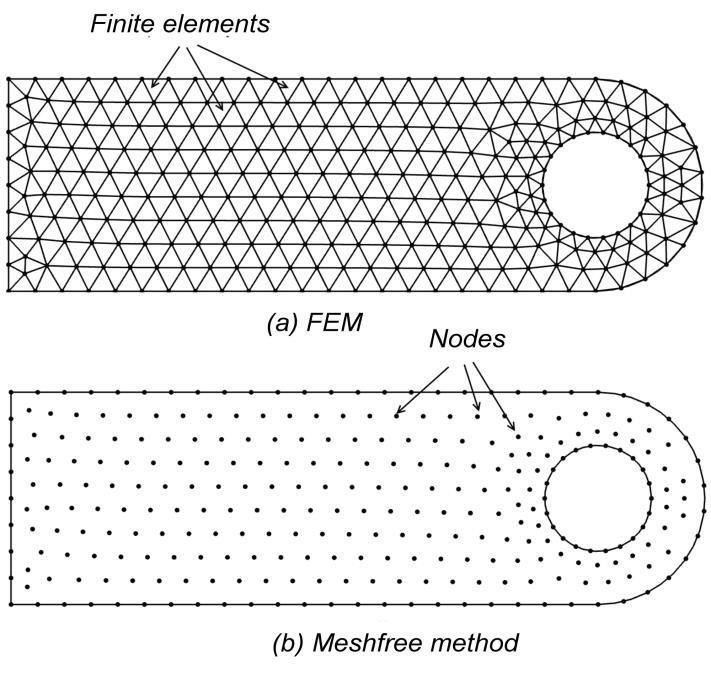
\includegraphics[width=11cm]{mesh_vs_meshfree.png}
	\caption{A comparison between a mesh-based and a mesh-free method. The upper model (a) is discretised into a mesh using nodes and elements, while the lower model (b) is discretised into a set of particles using only nodes \cite{kalutskiy_meshfree_2021}.}
	\label{fig:mesh_vs_meshfree}
\end{figure}

 Mesh-based methods are very well-established due to their relatively long history, and a variety of well-supported and well-validated software is available -- particularly for the finite element method. However, the meshing process is computationally expensive, which is of particular concern for crack propagation analysis -- where multiple steps of re-meshing may be required as the crack advances. This has been somewhat mitigated by the use of improvements to the original finite element method -- such as the extended finite element method (XFEM), which uses enriched elements near the crack tip to attempt to accurately capture the singularity and model its growth without re-meshing \cite{fries_extendedgeneralized_2010-1}. However, these enriched methods are more complex and less well-supported in terms of available software, and can lead to numerical instability and a loss of convergence if correct modelling approaches are not followed \cite{feng_past_2023}.

Mesh-free methods forgo the use of a mesh - instead discretizing the domain by splitting it into a series of independent points or particles. This approach provides some flexibility when analysing certain problems, as the particles are more free to undergo large displacements without requiring computationally expensive re-meshing. Smoothed-particle hydrodynamics (SPH) and the element-free Galerkin method (EFGM) have both been successfully applied to crack propagation analysis \cite{mu_improved_2023} \cite{belytschko_crack_1995}. However, the conventional Eulerian smoothed-particle hydrodynamics formulation suffers from tensile instability \cite{islam_total_2019}, and the standard enriched EFGM method is capable of modelling straight cracks only \cite{pant_novel_2013}. Mesh-free methods are also generally more computationally expensive than mesh-based methods \cite{liu_chapter_2014}, and at present are mainly limited to research rather than industrial applications.

The finite element method is by far the most commonly utilised method for performing structural analysis within industry, due to its versatility, reliability, long history of use, and the wide availability of mature software packages.  Therefore, the remainder of the literature review focuses on this method specifically.

\subsection{Element Formulations}

A key problem encountered when attempting to model a crack using the finite element method is the difficulty of accurately representing the singularity at the crack tip when discretising the structure. This leads to non-convergence of the results, since the polynomial interpolation functions used within standard elements are unable to accurately model the stress and strain singularities at the crack tip \cite{murti_universal_1986}. The most simple mitigation for this problem is to use a very fine mesh at the crack tip, which has been shown to be able to recover the full convergence of the finite element method \cite{fried_best_1972}.  However, increasing the mesh density also increases the solution time of the problem.

\begin{figure}[H]
	\centering
	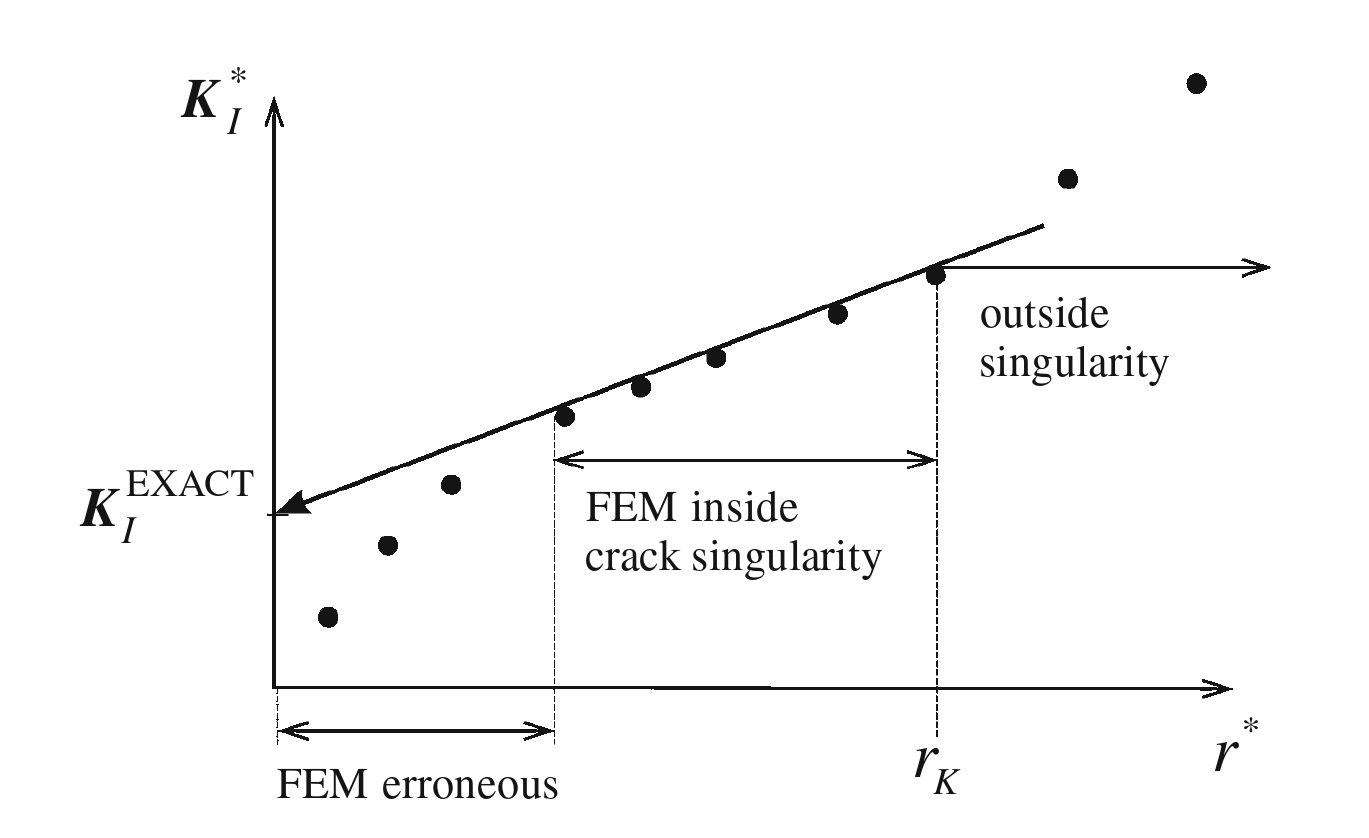
\includegraphics[width=10cm]{fem_linear_interpolation_kuna.png}
	\caption{Diagram of the validity range of SIFs obtained using a fine mesh of regular standard elements to model a crack\ \cite{kuna_finite_2013}.}
	\label{fig:fem_linear_interpolation_kuna}
\end{figure}

The alternative method of modelling the crack tip singularity is the use of specialised crack-tip elements, in which the shape functions contain singular crack-specific functions. These elements are used to model the area directly around the crack tip, while conventional elements are used to model the rest of the structure \cite{kuna_finite_2013}. The most commonly used of these is the quarter-point element (QPE), in which the mid-side nodes along the two edges intersecting the crack-tip are moved from the half-point of the edge to the quarter-point -- closer to the crack tip. These are relatively simple to implement for triangular elements, but more complex to implement for tetrahedral elements. However, quarter-point tetrahedral elements have been implemented successfully by separating them into corner-based or edge-based elements, depending on how they intersect the crack tip \cite{nejati_use_2015}.
	
\subsection{Stress \& Displacement Extrapolation}

A method of calculating the stress intensity factor by extrapolating the stresses or displacements near the crack tip was first proposed by Chan in 1970\ \cite{chan_finite_1970}. This method is based on the correlation of the stresses and displacements obtained from finite element results to analytical equations for the crack tip stress and displacement fields. For plane strain, this relationship is given by Equation \ref{eq:disp_extrap} \cite{anderson_fracture_2017}.

\begin{equation}
    K_I = \lim_{r\rightarrow0} \left[\frac{E u_y}{4} \sqrt{\frac{2 \pi}{r}} \right]\ \ \ \ (\theta = \pi)
    \label{eq:disp_extrap}
\end{equation}

\begin{itemize}
	\item $K_I$ is the Mode I stress intensity factor.
	\item $E$ is the elastic modulus of the material.
	\item $u_y$ is the crack opening displacement.
	\item $r$ and $\theta$ make up a polar coordinate system, with $r=0$ at the crack tip.
\end{itemize}

This equation relies on the fact that the stress intensity factor is related to both the applied stress and the distance from the crack tip, as illustrated in Equation \ref{eq:k_i}. Therefore, if the stresses and displacements near the crack tip (at some value of $r$) can be accurately calculated, they can by extrapolated to the crack tip -- where $r=0$ -- in order to calculate the stress intensity factor. More accurate results are generally obtained by extrapolating the displacements rather than the stresses, since stresses become singular as $r\rightarrow0$, while displacements are proportional to $\sqrt{r}$. This means that the displacement field is smoother and thus less sensitive to mesh discretisation errors compared to the stress field. The key disadvantage of this method is that it requires a very fine mesh around the crack tip, and is very sensitive to the nodes which are selected to perform the extrapolation. These methods have largely been superseded by energy-based methods, which are generally more robust in practical applications \cite{anderson_fracture_2017}.

\subsection{Virtual Crack Extension}\label{sec:vce}
    
The virtual crack extension (VCE) method is an energy-based approach first described by Parks\ \cite{parks_virtual_1977} and Hellen\ \cite{hellen_method_1975} in the late 1970s. The basis of the method is the simulation of a small virtual extension of a crack, from which the rate of change in potential energy can be calculated. The total potential energy of the system is given by Equation \ref{eq:vce}.

\begin{equation}
    \Pi = \frac{1}{2} \textbf{u}^T \textbf{K} \textbf{u} - \textbf{u} \textbf{F}
    \label{eq:vce}
\end{equation}

\begin{itemize}
	\item $\Pi$ is the total potential energy.
	\item $\textbf{u}$ is the displacement vector.
	\item $\textbf{K}$ is the stiffness matrix.
	\item $\textbf{F}$ is the externally applied force.
\end{itemize}

If this expression is differentiated with respect to a small extension of crack length $a$, and the assumption is made that the external forces (\textbf{$F$}) do not change, Equation \ref{eq:vce} can be simplified to produce Equation \ref{eq:vce_2}.

\begin{equation}
    G = -\frac{\partial \Pi}{\partial a} = \frac{1}{2} \textbf{u}^T \frac{\partial \textbf{K}}{\partial a} \textbf{u}
    \label{eq:vce_2}
\end{equation}

It can therefore be observed that the strain energy release rate $G$ is dependent on the derivative of the stiffness matrix $\textbf{K}$, based on the change in stiffness between the initial crack state and the extended crack state. The displacement solution $\textbf{u}$ is only required for the initial state, simplifying the analysis. In order to calculate the change in stiffness, a small subset of elements around the crack tip can be shifted by the change in crack length ($\Delta a$) in order to change the stiffness matrix slightly in the region of the crack tip \cite{anderson_fracture_2017}. The key advantage of this approach is that it can be performed in the post-processing stage, without requiring another finite element analysis run to be performed. This method is more accurate than the displacement extrapolation method, and a good level of accuracy can be obtained with the use of standard elements. However, some numerical sensitivity is present in terms of the choice of $\Delta a$. The most significant disadvantage of this method is that it is not possible to separate the stress intensity factors of each loading mode ($K_I$, $K_{II}$, $K_{III}$) directly, and an additional step must be performed in order to decompose the results. This significantly reduces the utility of this method \cite{kuna_fe-techniques_2013}.

\begin{figure}[H]
    \centering
    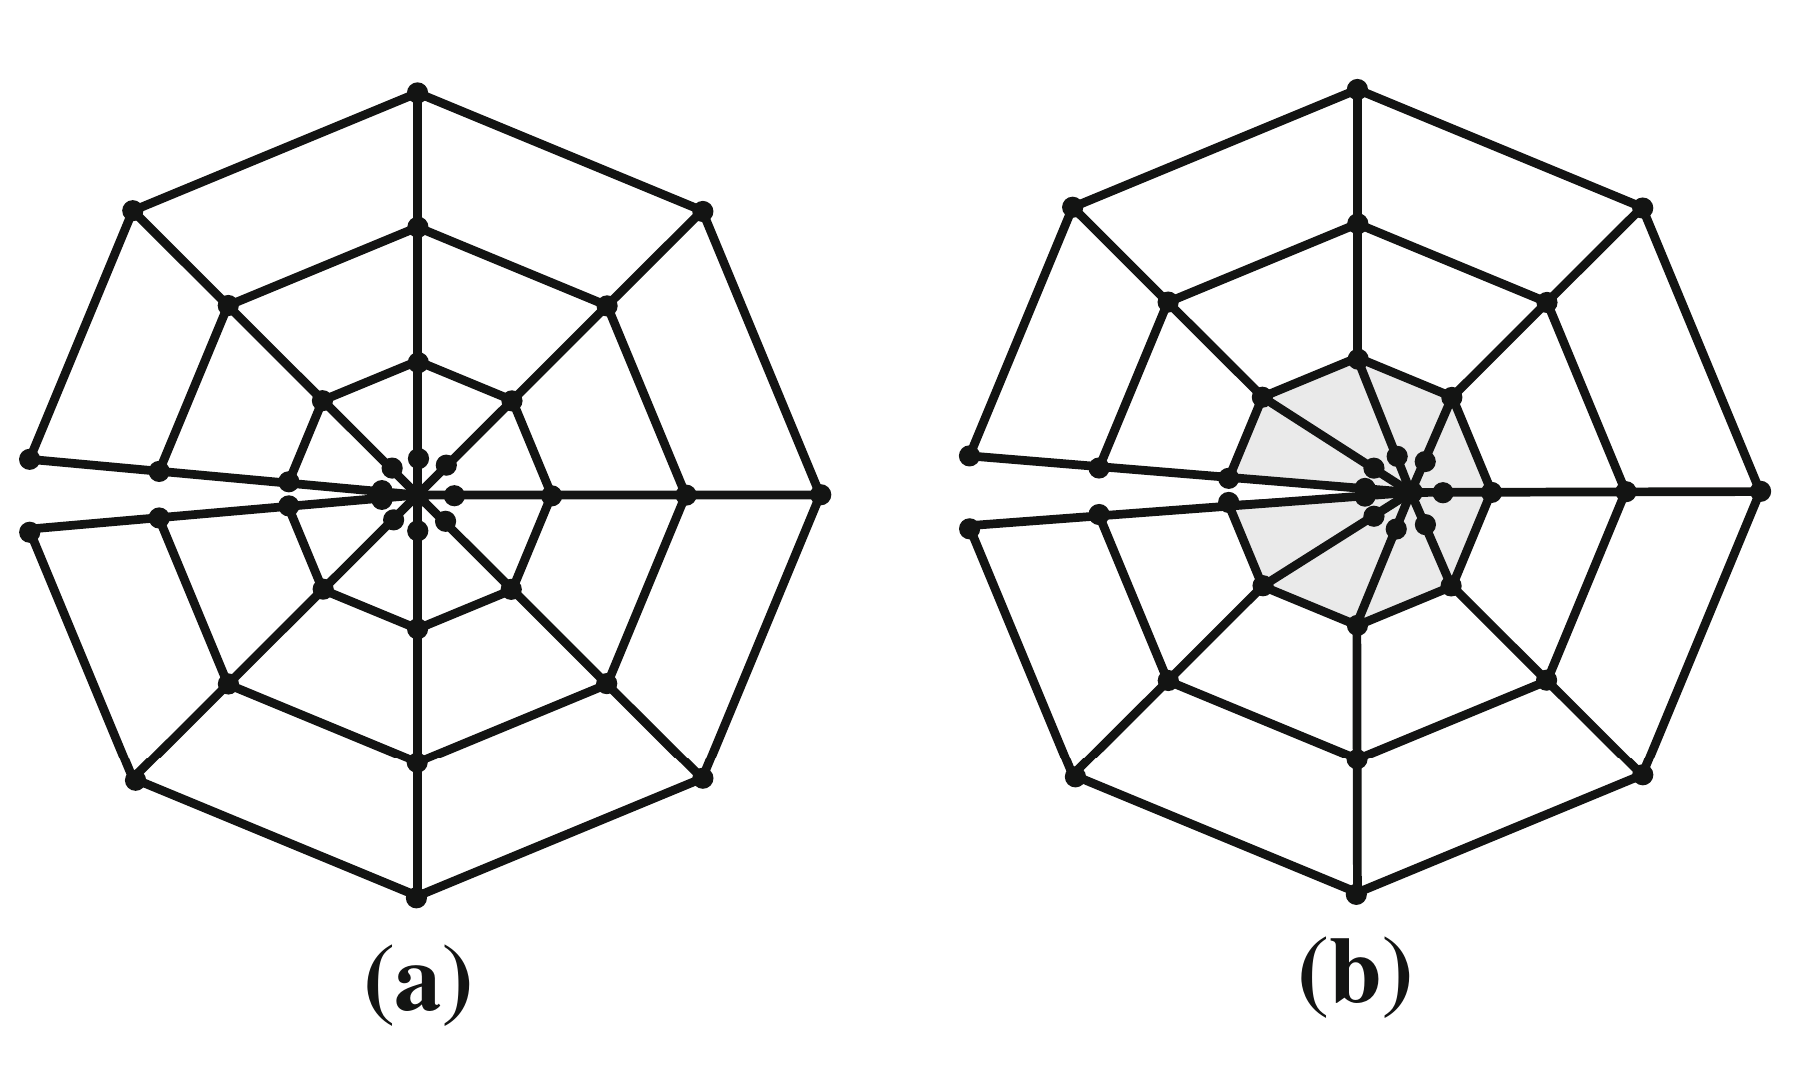
\includegraphics[width=10cm]{crack_extension_kuna.png}
    \caption{Diagram of the virtual crack extension technique. The first image (a) shows the initial crack state, while the second (b) shows the virtual extension of the crack tip elements (highlighted in colour) \cite{kuna_fe-techniques_2013}.}
    \label{fig:crack_extension_kuna}
\end{figure}

\subsection{Virtual Crack Closure}

The virtual crack closure technique (VCCT) was first described by Rybicki and Kanninen -- again in the 1970s. It is an energy-based method which utilises Irwin's crack closure integral -- which relates the energy release rate to the stresses and displacements near the crack tip -- and adapts it for use as a computational method. In the simple case, this involves running two finite element analyses, whereby the crack is extended a small amount by separating the mesh near the crack tip. The work required to close the crack back to its initial state can then be determined by using Irwin's crack closure integral to calculate the energy release rate $G$\ \cite{milne_numerical_2003}. This method was extended in order to develop the modified crack closure integral (MCCI) method\ \cite{rybicki_finite_1977}. With this method, only a single finite element analysis is required, with the crack in its initial state. The displacements after the crack has been extended can then be approximated via interpolation, assuming that a small extension of the crack does not significantly change the loading state at the crack tip\ \cite{kuna_fe-techniques_2013} A diagram of this process is presented in Figure \ref{fig:crack_closure_milne}.

\begin{figure}[H]
    \centering
    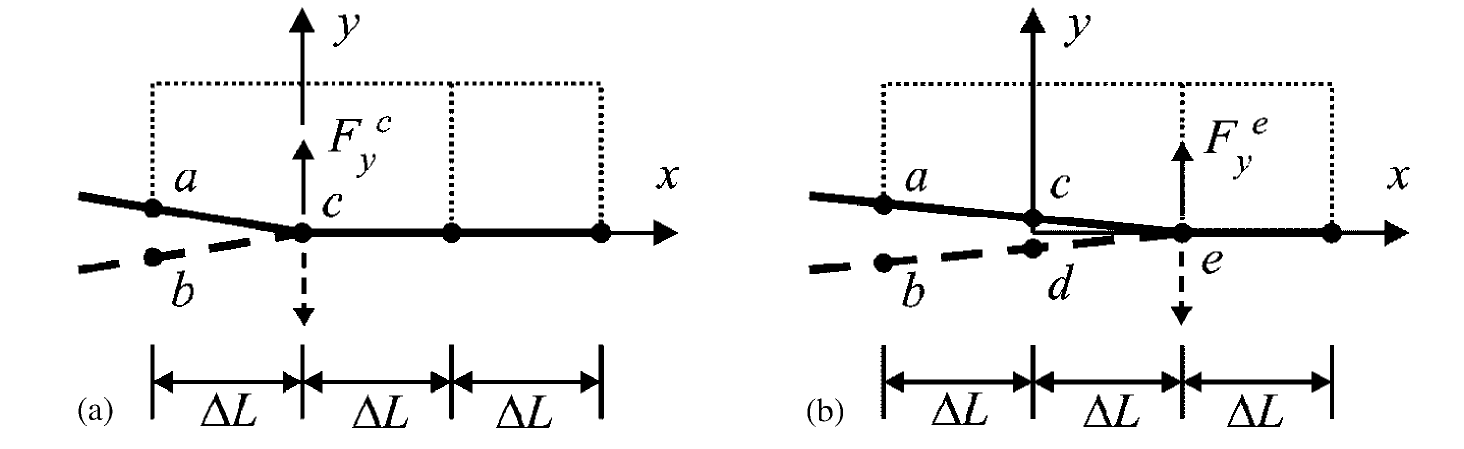
\includegraphics[width=14cm]{crack_closure_milne.png}
    \caption{Diagram of the MCCI technique. The first analysis (a) shows the initial crack state, while the second (b) shows the state after the crack has been extended. The displacements at $c$ and $d$ in (b) can be approximated by using the displacements at $a$ and $b$ in (a), without requiring a second analysis to be performed\ \cite{milne_numerical_2003}.}
    \label{fig:crack_closure_milne}
\end{figure}

\subsection{Equivalent Domain Integral}\label{sec:equiv_domain}

As discussed in \S\ref{sec:j-integral}, the J-integral is a path-independent contour integral around the tip of a crack, which can be used to determine the stress intensity factor. The standard contour-based formulation of the J-integral is relatively difficult to implement using the finite element method. The options for defining the contour are either to define the contour through a set of nodes, or to define the contour as a circle and allow it to pass through elements when required. Defining the contour through nodes only potentially can produce a highly distorted contour unless a structured mesh is used, while defining it to pass through elements necessitates the interpolation of values within the element. Both of these approaches can lead to inaccurate results if not done carefully.

Shih et al. \cite{shih_energy_1986} introduced an alternative method -- known as the equivalent domain integral (EDI) method -- where the contour integral was converted into a domain integral using the divergence theorem. This allowed the line integral to be restated in terms of area, converting the original equation for the J-integral (Equation \ref{eq:j-integral}) into Equation \ref{eq:j_integral_2d}.

\begin{equation}\label{eq:j_integral_2d}
	J = \int_A \left[\sigma_{ij}\frac{\partial u_i}{\partial x_1} - W\,\delta_{1j}\right]\frac{\partial q}{\partial x_j}\, dA
\end{equation}

\begin{itemize}
	\item \(u_i\) is the displacement field.
	\item \(\sigma_{ij}\) is the stress tensor.
	\item \(W\) is the strain energy density.
	\item \(\delta_{1j}\) is the Kronecker delta.
	\item \(q\) is a smooth weight function that equals 1 at the inner boundary of the integral domain, and decays to 0 at the outer boundary of the integral domain.
	\item \(A\) is the area over which the integration is performed. For the 3D analysis, $V$ was substituted here instead, which was the volume over which the integration was performed.
\end{itemize}

The conversion of the contour integral into a domain integral necessitated the introduction of a smooth weight function. This is an arbitrary function that is equal to 1 at the inner boundary of the integral domain, equal to 0 at the outer boundary of the domain, and decays smoothly throughout the domain. Spreading the integral across a larger domain of elements vs a single contour reduces the sensitivity of the results to local mesh discontinuities, while the weight function acts to ensure that elements closer to the crack tip are more strongly represented within the J-integral.

The equivalent domain integral method is closely related to the virtual crack extension method discussed in \S\ref{sec:vce}. While the virtual crack extension method explicitly calculates the change in potential energy caused by the extension of the crack, the equivalent domain integral method implicitly performs the same calculation via the use of the weight function. The equivalent domain integral can also be extended to three-dimensions by conversion to a volume integral, which is created by extending the area integral along the crack tip, creating a cylinder over which to perform the integration. This is presented in Figure \ref{fig:integral_domains}.

\begin{figure}[H]
	\centering
	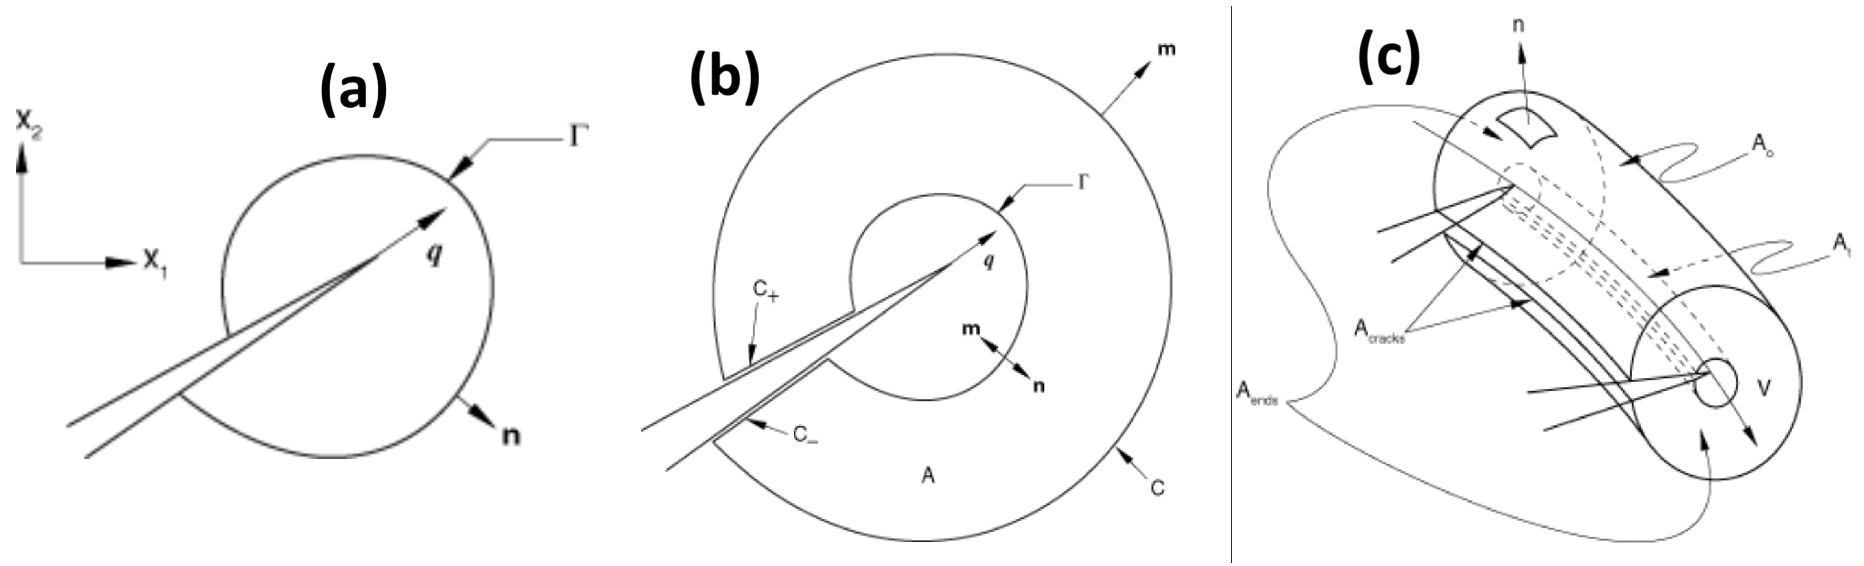
\includegraphics[width=\textwidth]{contour_domain.png}
	\caption{Diagram visualising the different J-integral formulations. The contour integral in 2D (a) is shown, along with the domain integral in both 2D (b) and 3D (c) \cite{systemes_2161_nodate}.}
	\label{fig:integral_domains}
\end{figure}

\section{Summary}

This literature review began with a discussion of aerospace fatigue and damage tolerance certification requirements (\S\ref{sec:cert_req}), which highlighted the importance of understanding crack initiation and propagation when designing safe and reliable aircraft structures. The available methods for fatigue and damage tolerance analysis were then discussed in \S\ref{sec:fdt_analysis}. The key aim of this section was to emphasise the importance of being able to accurately calculate crack propagation lives in order to set safe inspection thresholds and intervals. \S\ref{sec:lefm} then went on to review the key theoretical concepts underpinning damage tolerance analysis, and discussed key concepts such as the stress intensity factor and the J-integral. The final section (\S\ref{sec:comp_fracture}) explained the difficulties in calculating these parameters analytically for three-dimensional crack configurations, and provided an overview of some computational methods which were able to accomplish this task. The overall project was therefore put into context. Aerospace certification requirements necessitate the requirement of accurate crack propagation lives. These can be obtained by calculating the stress intensity factor for the crack, and using as an input for the Paris-Erdogan equation. However, obtaining the stress intensity factor for three-dimensional configurations requires a laborious manual meshing process. Therefore, a need has been demonstrated for a piece of software which is capable of accurately calculating the stress intensity factor for a three-dimensional crack, using an unstructured mesh which can be generated quickly and automatically. At present, such capabilities are limited to expensive commercial software or proprietary company tools. Therefore, this project aims to fill that gap by developing such a piece of software. The implementation of this software is discussed in the following section.
